\chapter{Divulgación y software libre}
\label{chap:aplicacion_web}

\lettrine{C}{lúpiter} sirve para explicar el funcionamiento de los superordenadores. Para este cometido se desarrolla una aplicación web, el \textit{dashboard} de ahora en adelante, que aloja vídeos divulgativos y una herramienta para realizar demostraciones en vivo.

\section{Vídeos divulgativos}
En este dashboard se pueden encontrar dos vídeos didácticos y divulgativos. El primero de ellos trata de manera muy superficial el concepto de superordenador, se aporta contexto histórico y cifras acerca de lo enorme de estas máquinas de cómputo, y cuales son y han sido sus utilidades y logros. Tras ello se realiza una descripción de Clúpiter y sus partes fundamentales, y se relacionan con sus análogos en un supercomputador real. Este vídeo está claramente orientado a educar en conceptos muy básicos acerca del \acrshort{hpc}, pero también a motivar e inspirar a futuros ingenieros. El vídeo en cuestión puede encontrarse en la dirección \url{https://youtu.be/o76-VP6WFCo}.

El segundo vídeo, ya más técnico, habla mediante animaciones ilustradas a mano acerca del funcionamiento interno de un supercomputador, su necesidad en el día a día, y las restricciones que tienen que superar los programas paralelos, mediante analogías y evitando el tecnicismo. Tras ello, se da una breve introducción a las operaciones más básicas de \acrshort{mpi}, y se finaliza el vídeo con una cuestión acerca de cómo ordenar diez mil hojas a mano entre varias personas, un recurso que expositor podrá emplear si lo considera conveniente. Con esta tarea se pueden explicar de manera intuitiva, e incluso competiva, múltiples conceptos de computación. En concreto se pueden razonar los algoritmos de ordenación y visualizar de primera mano las restricciones de la programación paralela, incluyendo la ralentización que supone el acceso a red, o las diferencias de acceso a memoria uniforme (\acrshort{uma} o \acrlong{uma}) con respecto al no uniforme (\acrshort{numa} o \acrlong{numa}). Dicho vídeo se puede encontrar en la dirección \url{https://youtu.be/if0MWI_9xzM}.

Finalmente, destacar que estos vídeos, en su versión alojada en YouTube, cuentan con subtítulos en español en caso de que sean expuestos a personas con discapacidades auditivas.

\section{Dashboard}
El dashboard se ha programado empleando tecnologías web (HTML, CSS y JS), y todos los archivos \LaTeX, scripts, imágenes y recursos relacionados con este trabajo, pueden encontrarse en la dirección \url{https://github.com/forcegk/GEI_TFG} bajo licencia MIT, así como el propio código del dashboard, que se encuentra en la carpeta \texttt{app/node}. Este repositorio git es el que se ha empleado a lo largo de todo el desarrollo, y así puede comprobarse en el historial de commits. Debido a la naturaleza individual de un \acrshort{tfg}, no hay ningún especial gitflow ni colaboraciones de terceros incorporadas al desarrollo.

Varias imágenes de la página principal del dashboard se pueden ver a continuación en las Figuras \ref{fig:inicio_clupiter}, \ref{fig:monitorizacion_clupiter} y \ref{fig:agradecimientos_clupiter}.

\begin{figure}[h!]
  \centering
  \vspace{0.20cm}
  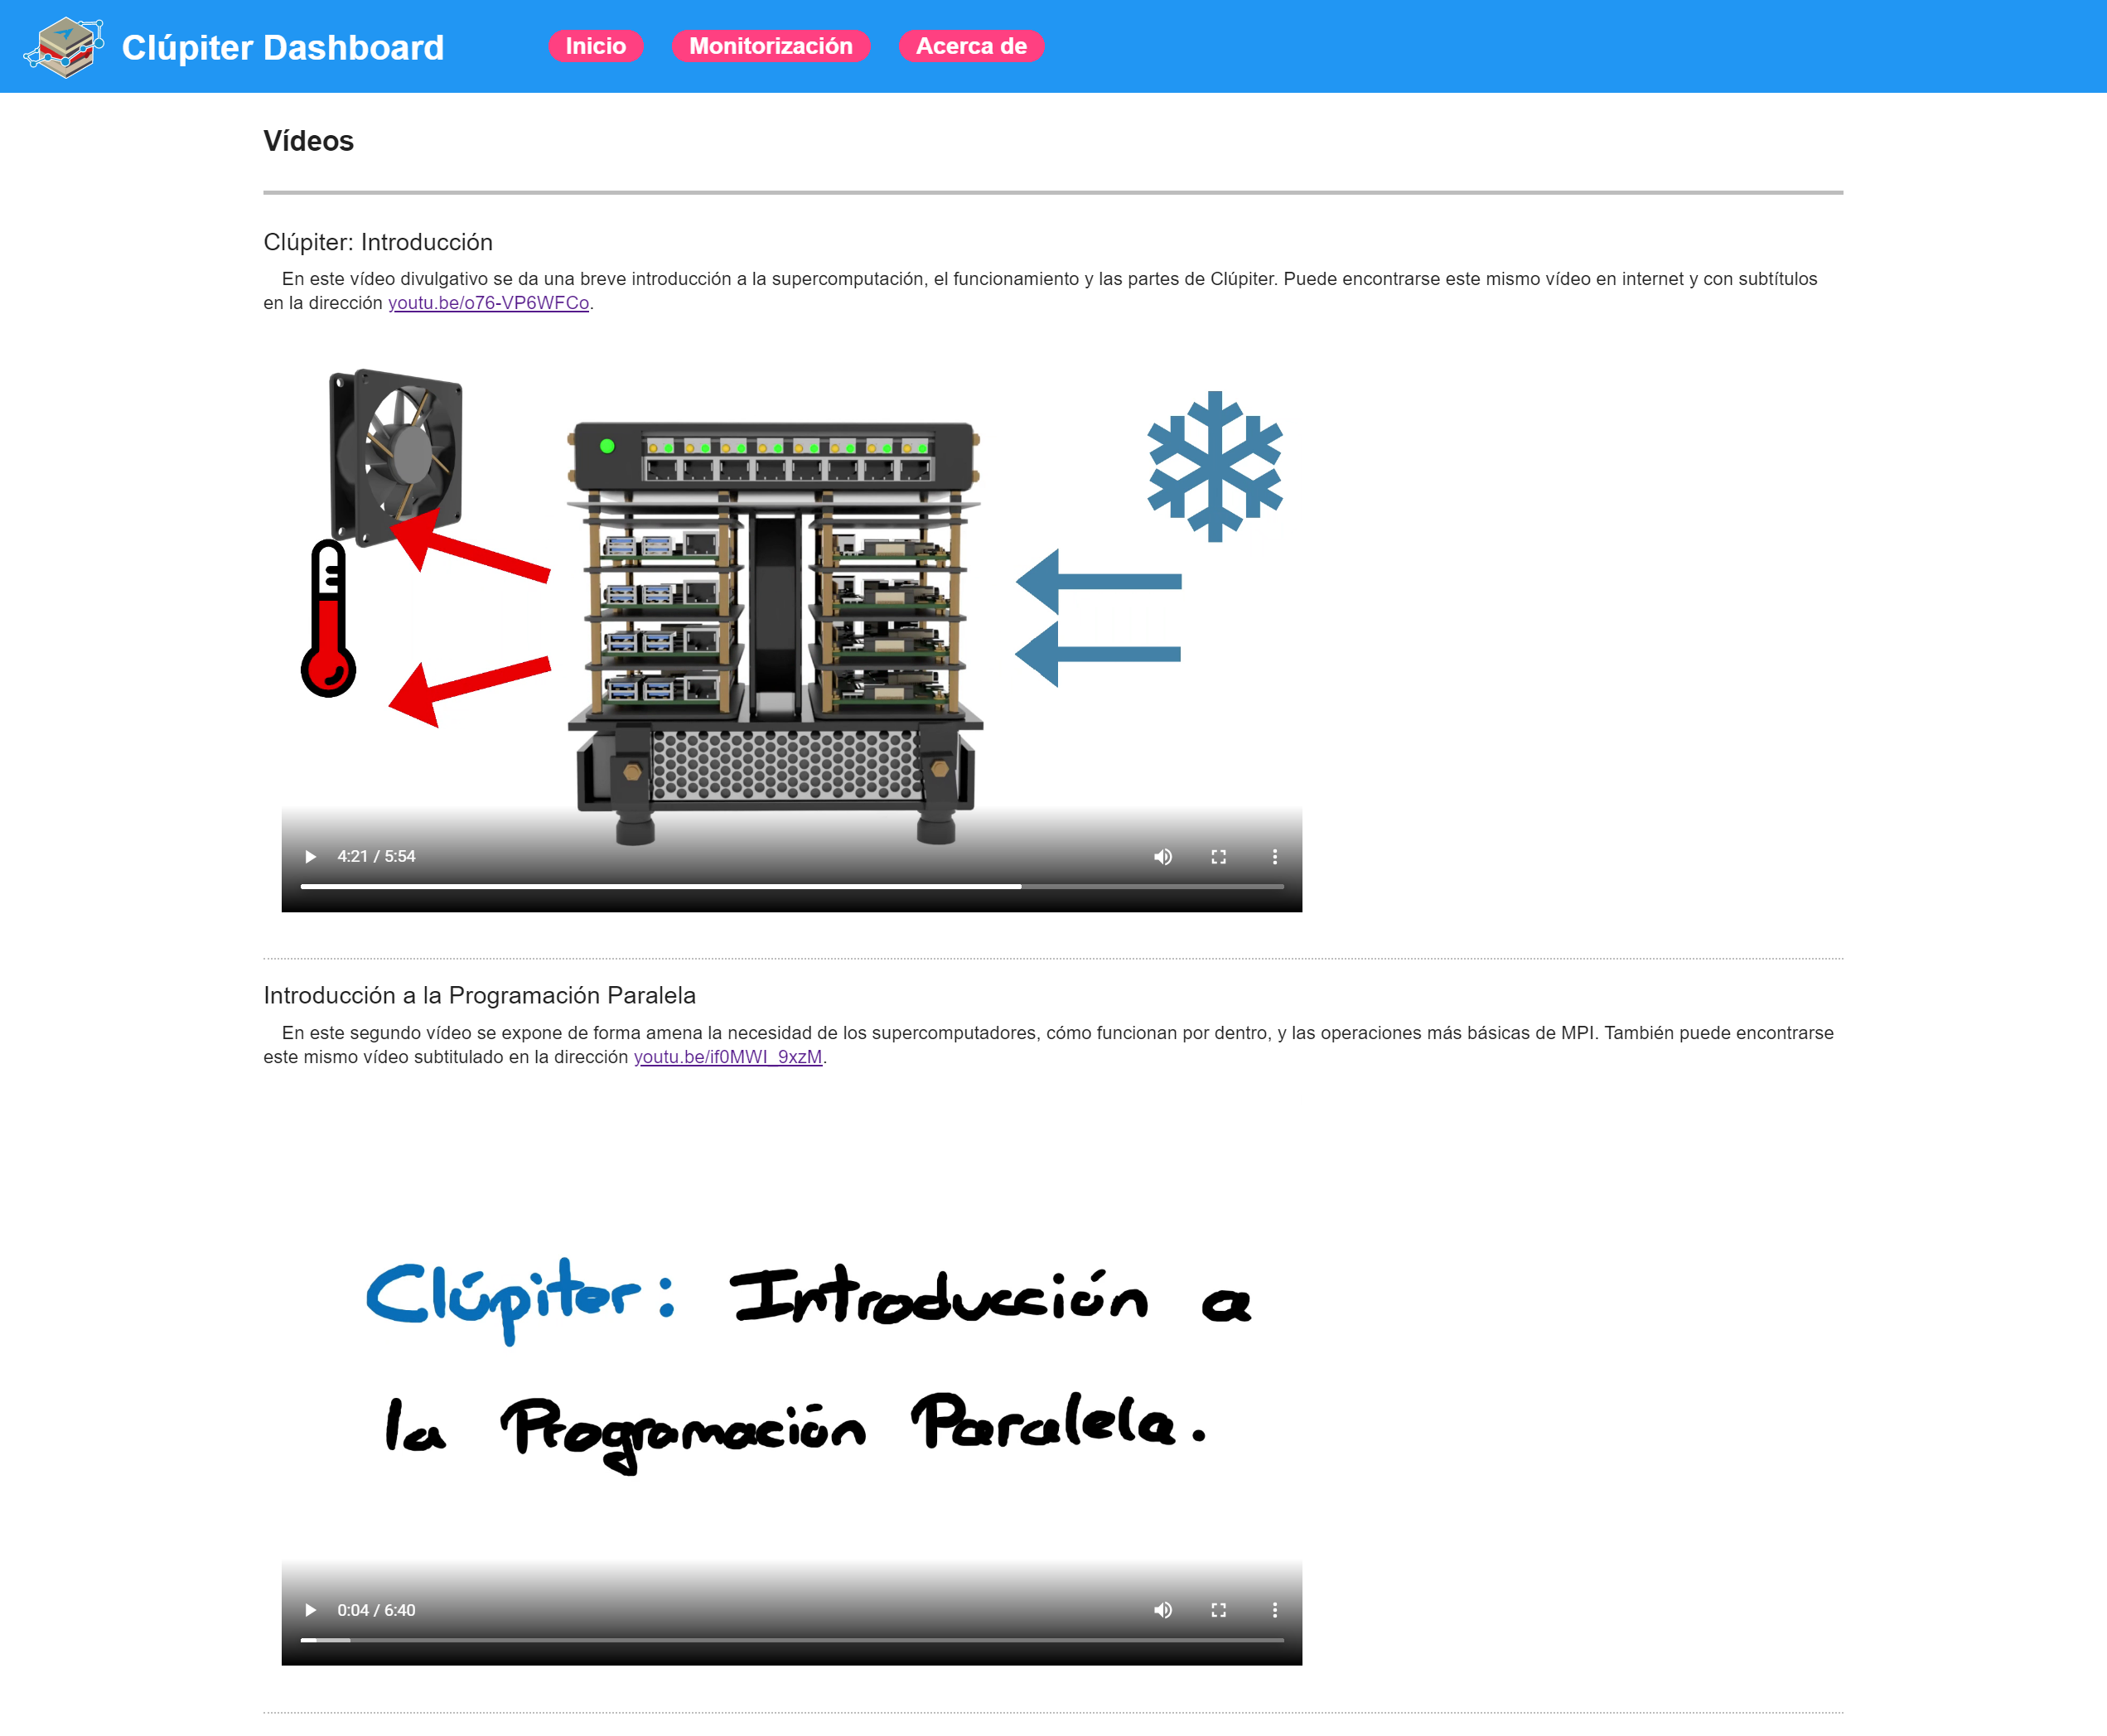
\includegraphics[width=0.98\textwidth]{img/dashboard/inicio.png}
  \caption{Página de inicio de Clúpiter}
  \label{fig:inicio_clupiter}
\end{figure}


\begin{figure}[h!]
  \centering
  \vspace{0.20cm}
  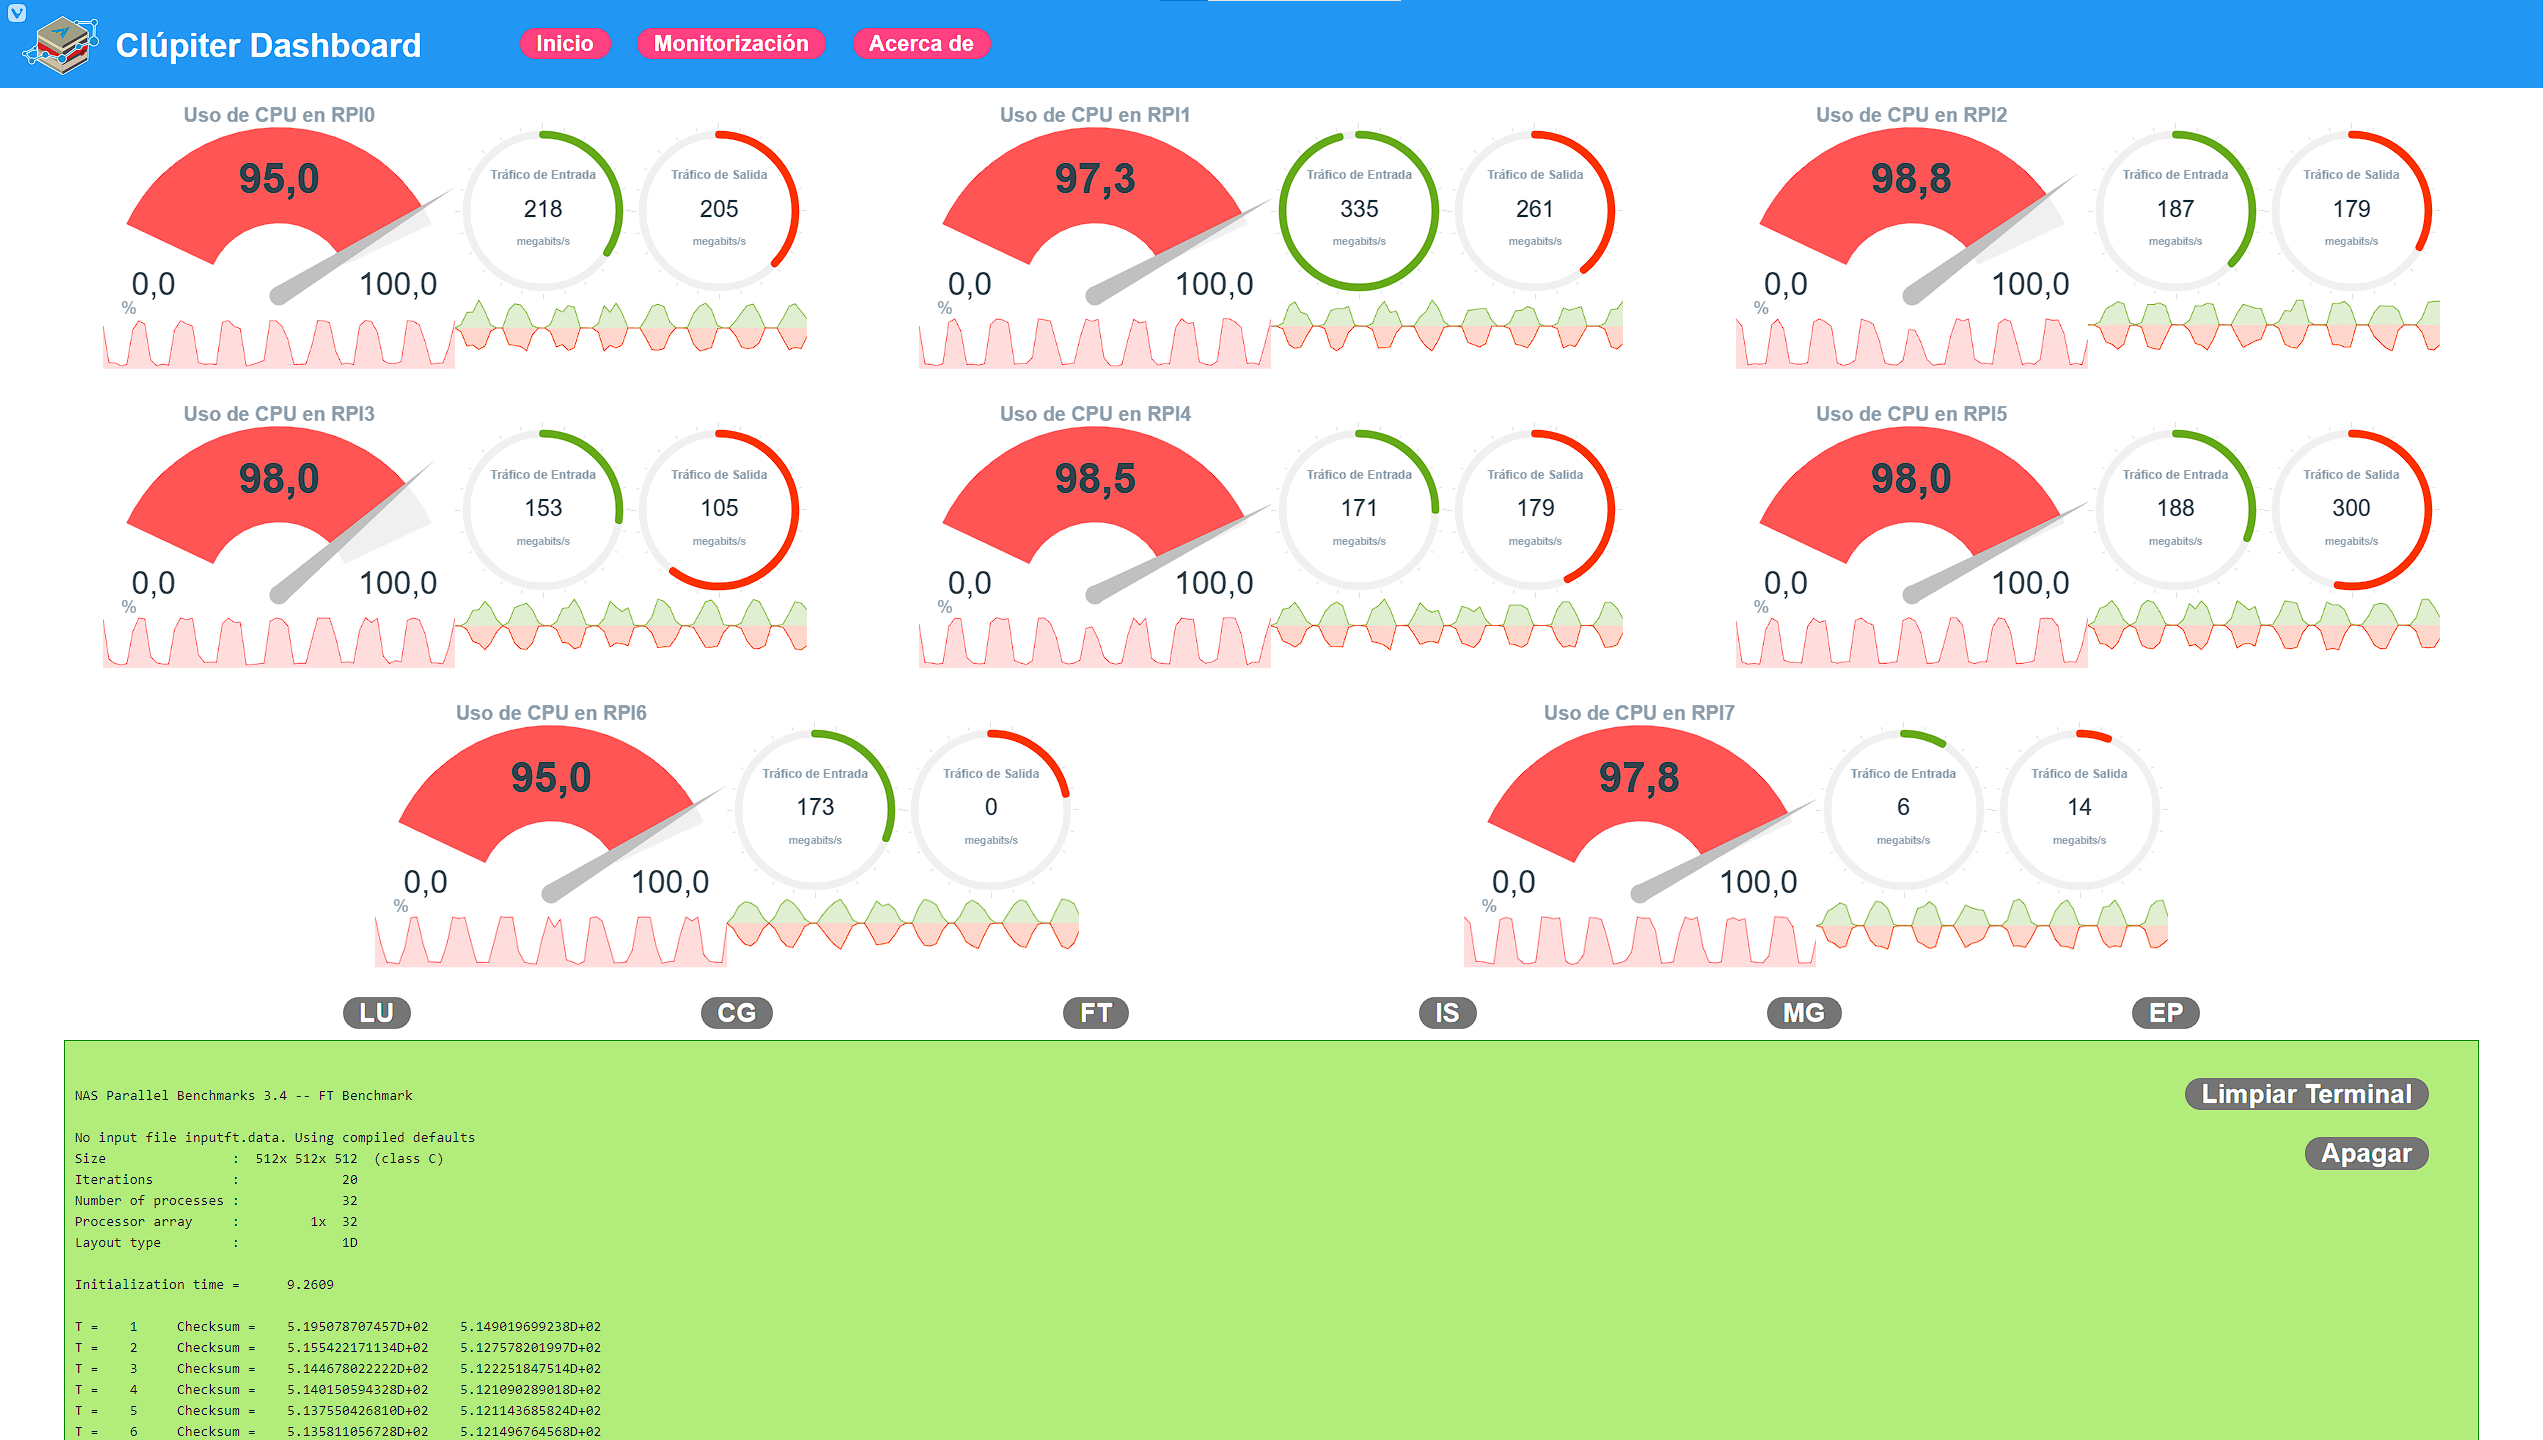
\includegraphics[width=0.98\textwidth]{img/dashboard/monitoring.png}
  \caption{Página de monitorización de Clúpiter}
  \label{fig:monitorizacion_clupiter}
\end{figure}

\begin{figure}[h!]
  \centering
  \vspace{0.20cm}
  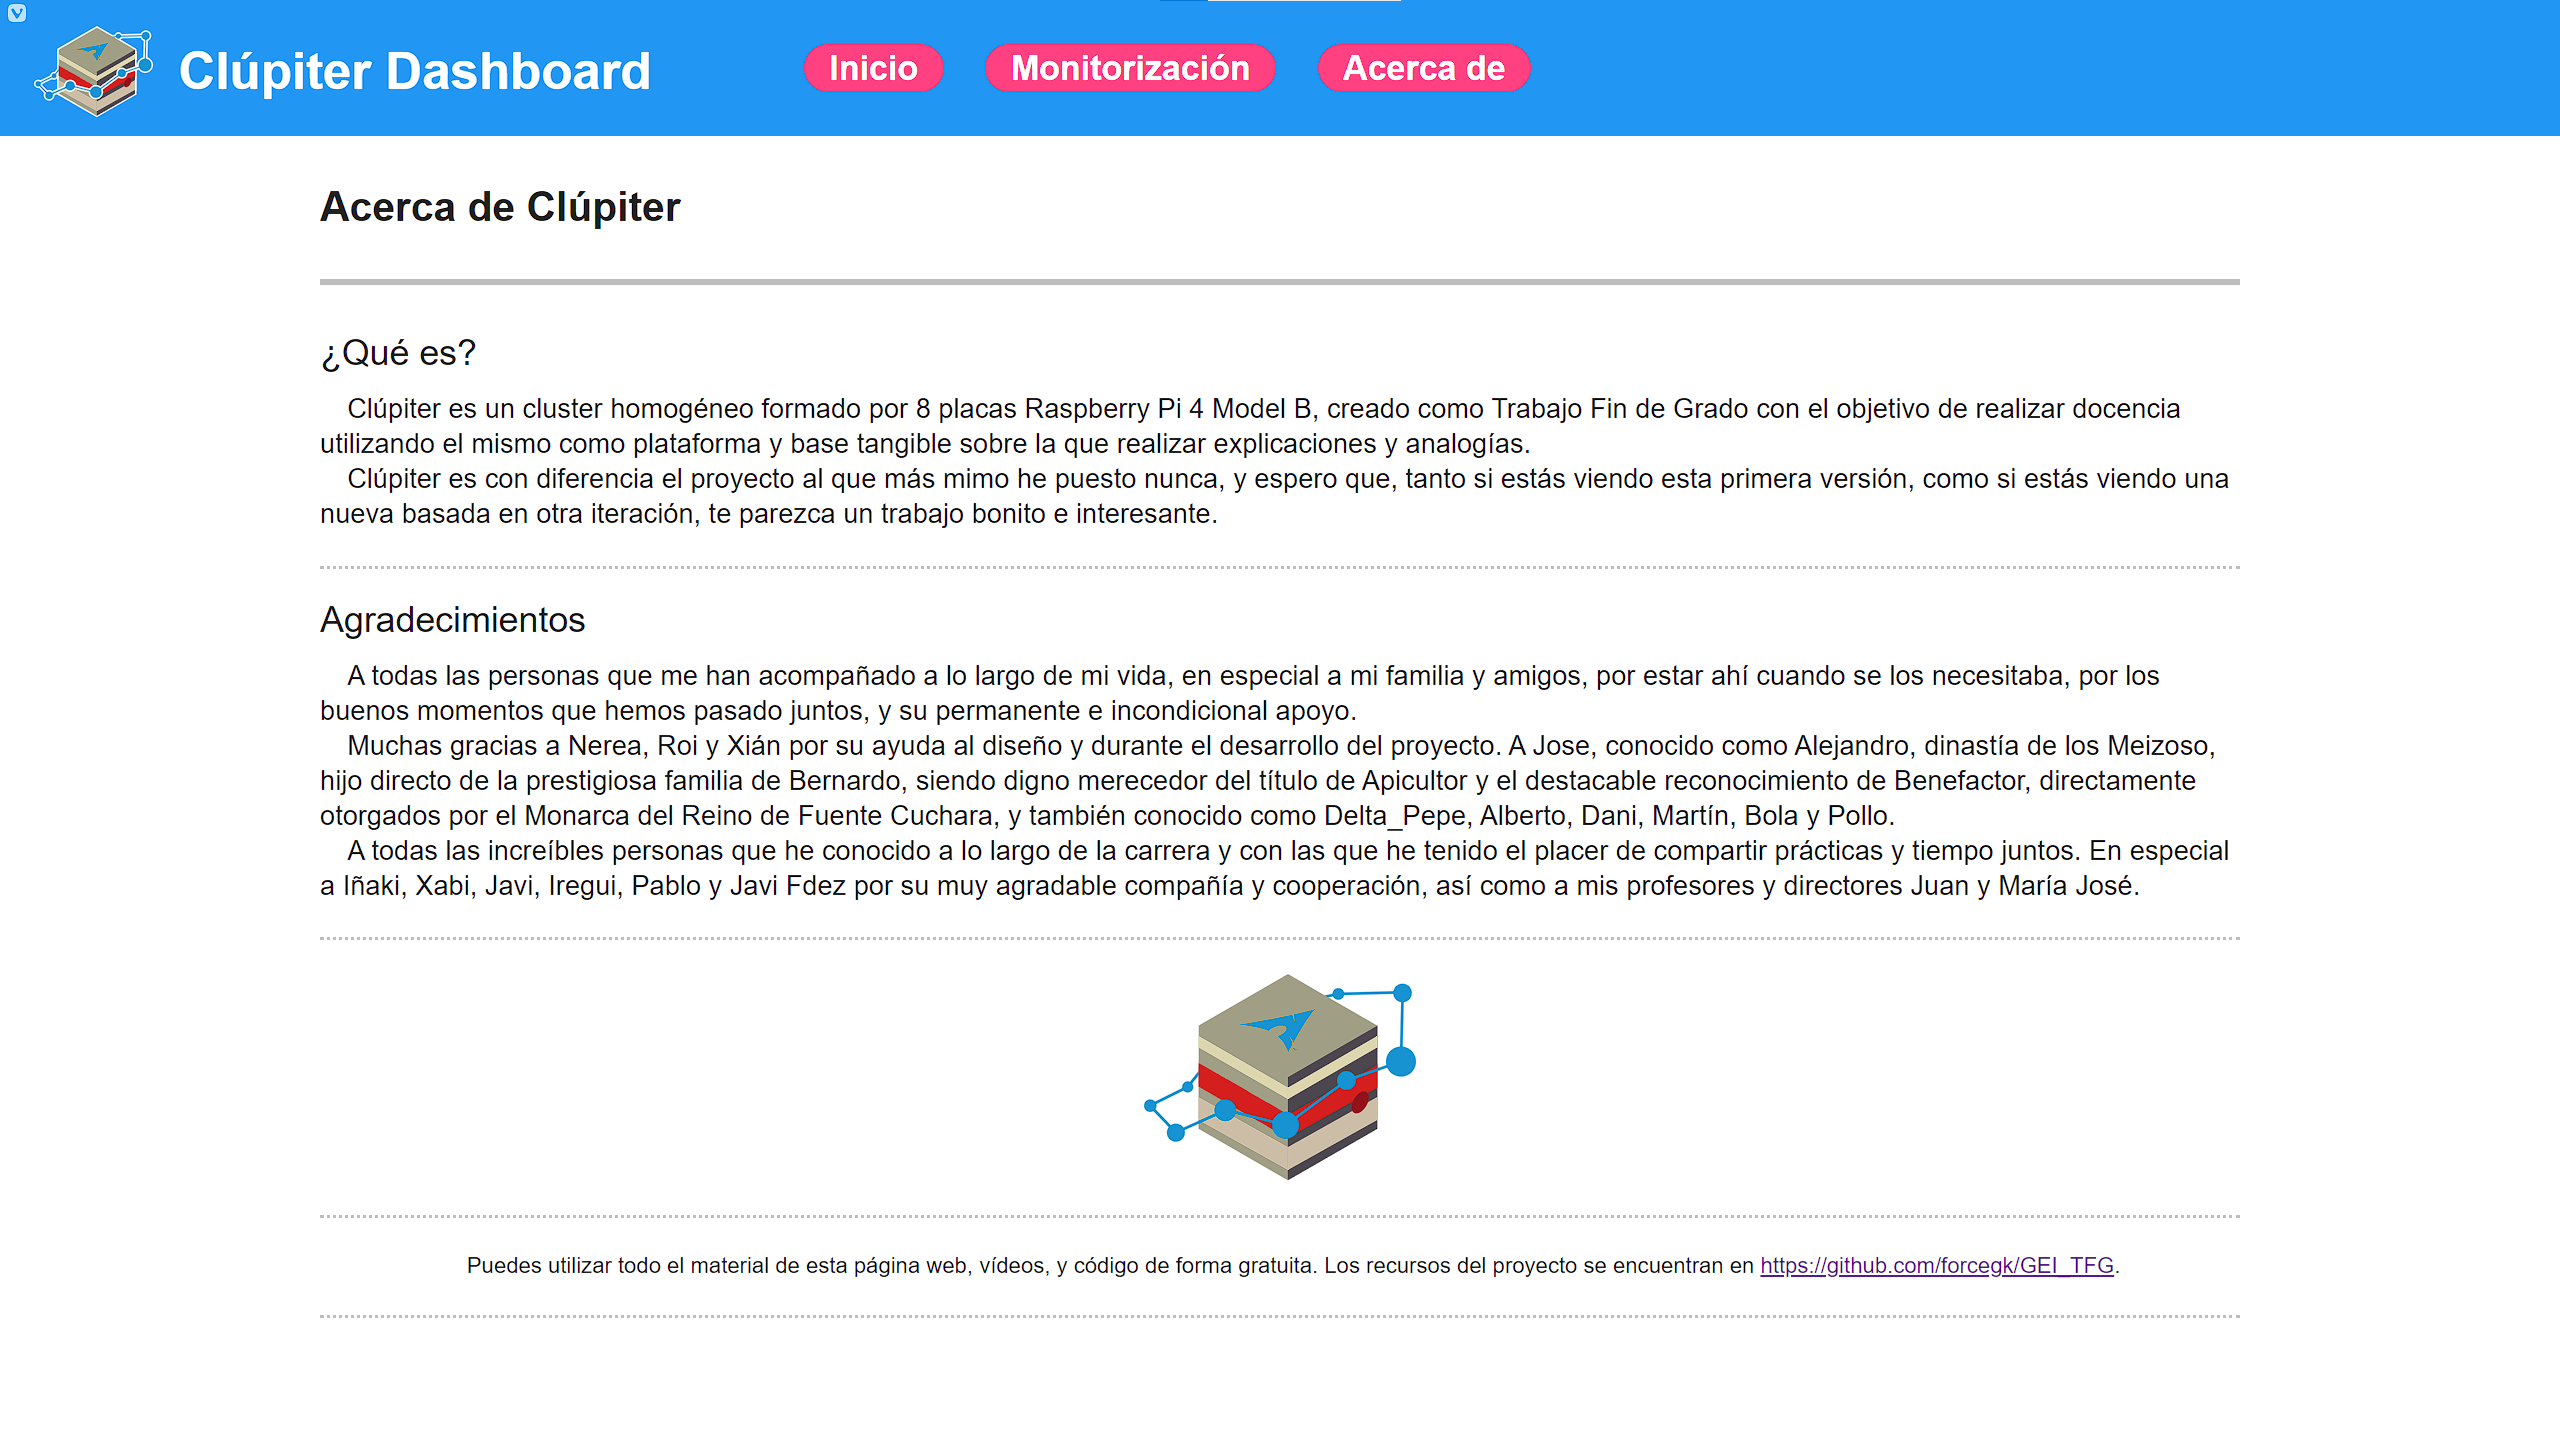
\includegraphics[width=0.98\textwidth]{img/dashboard/agradecimientos.png}
  \caption{Página de agradecimientos de Clúpiter}
  \label{fig:agradecimientos_clupiter}
\end{figure}
